\begin{frame}{Aufgabe}
	\visible<2->{
		\begin{itemize}
			\item Webserver für Most Useless Machine Ever!
		\end{itemize}
	}
	\begin{center}
		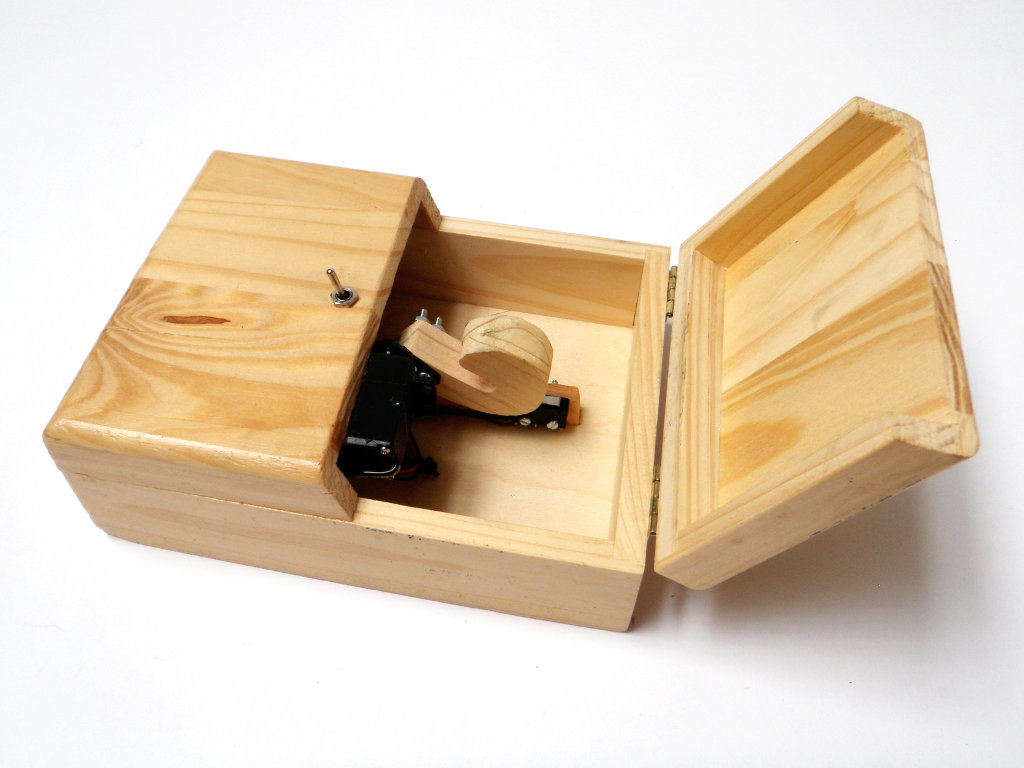
\includegraphics[height=4cm]{res/mume.jpg}
		\hcite{mumePic}
		\visible<2->{
			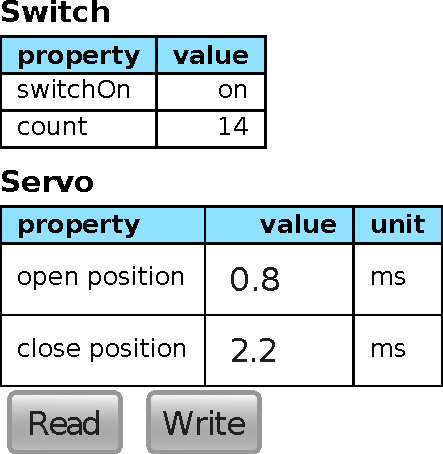
\includegraphics[height=4cm]{res/mumehtml.pdf}
		}
	\end{center}
\end{frame}

\begin{frame}{Vorgehen}
\tableofcontents
\end{frame}

\section{Hardware}

\begin{frame}{System}
	\begin{center}
		\begin{tabular}{cc}
			Bare Metal uC & GNU/Linux SOC \\
			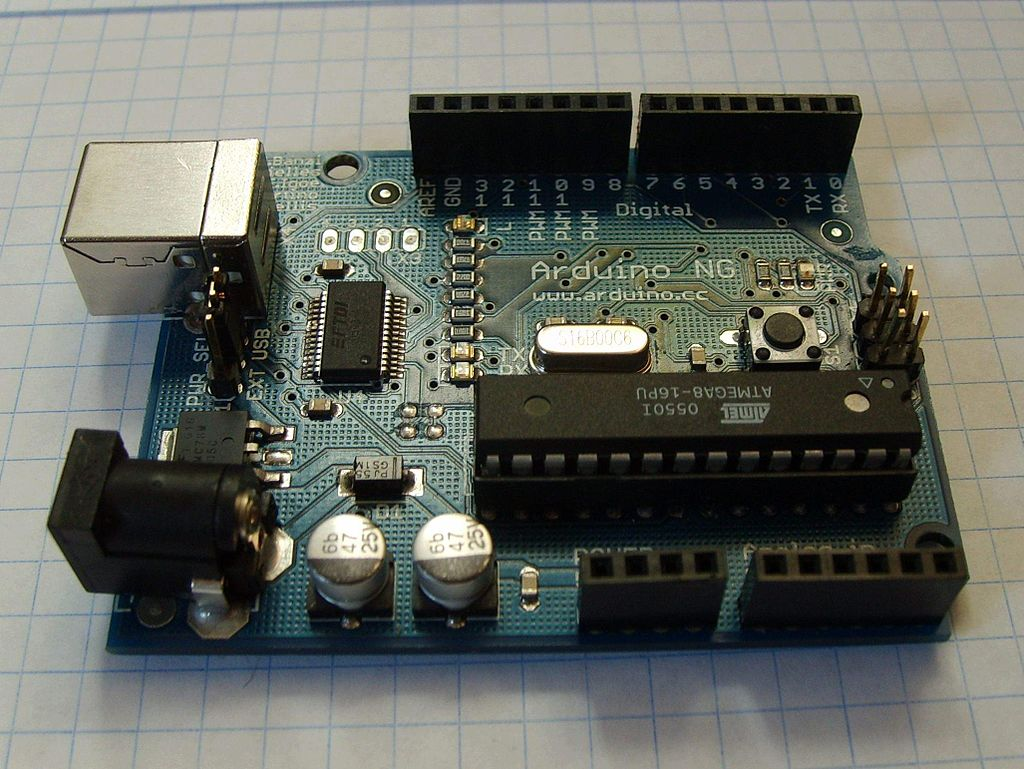
\includegraphics[height=3cm]{res/arduino.jpg} & 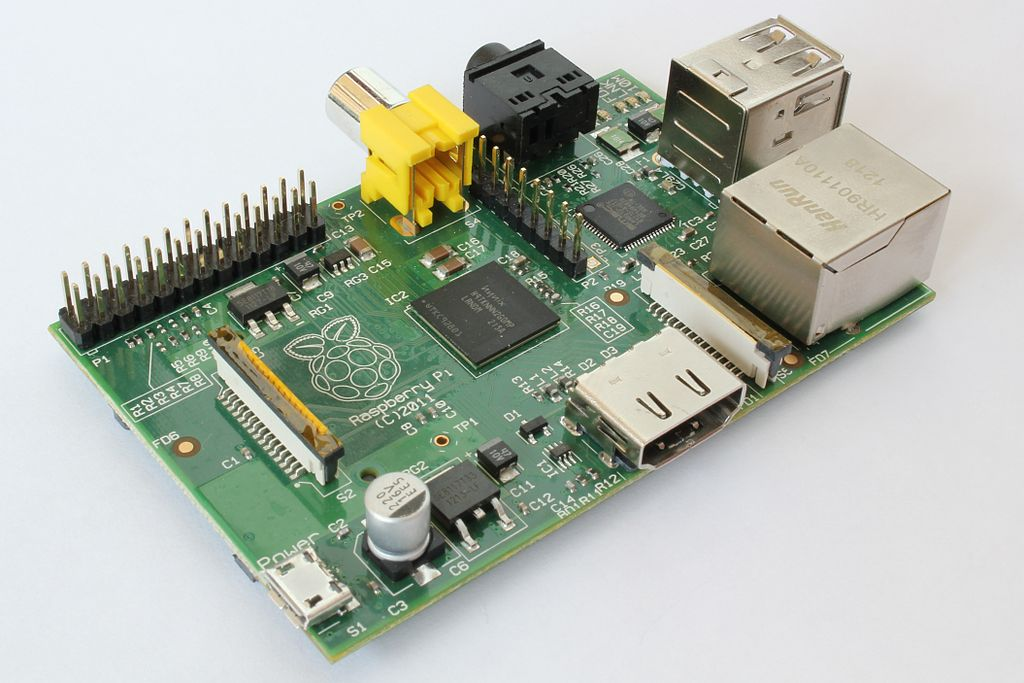
\includegraphics[height=3cm]{res/RaspberryPi.jpg}\hcite{raspberryPi} \\
			\only<handout>{
				Echtzeit & Memory und Prozess Management\\
				niedrige System-Komplexität & Treiber \& Protokolle\\
				keine Infrastruktur & hohe System-Komplexität
			}
		\end{tabular} 
	\end{center}
\end{frame}

\begin{frame}{Board}
	\begin{center}
		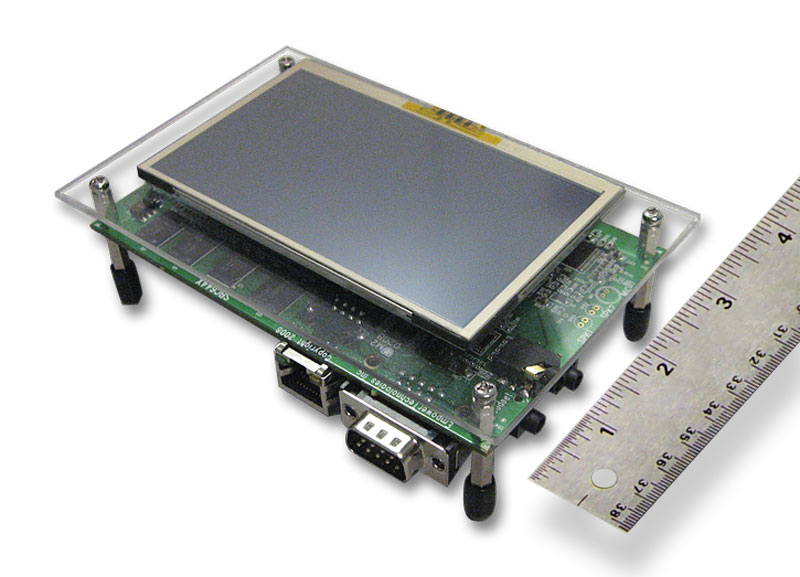
\includegraphics[height=2.7cm]{res/Development_Kit_EDK6446.jpg}\hcite{industrialBoard}
		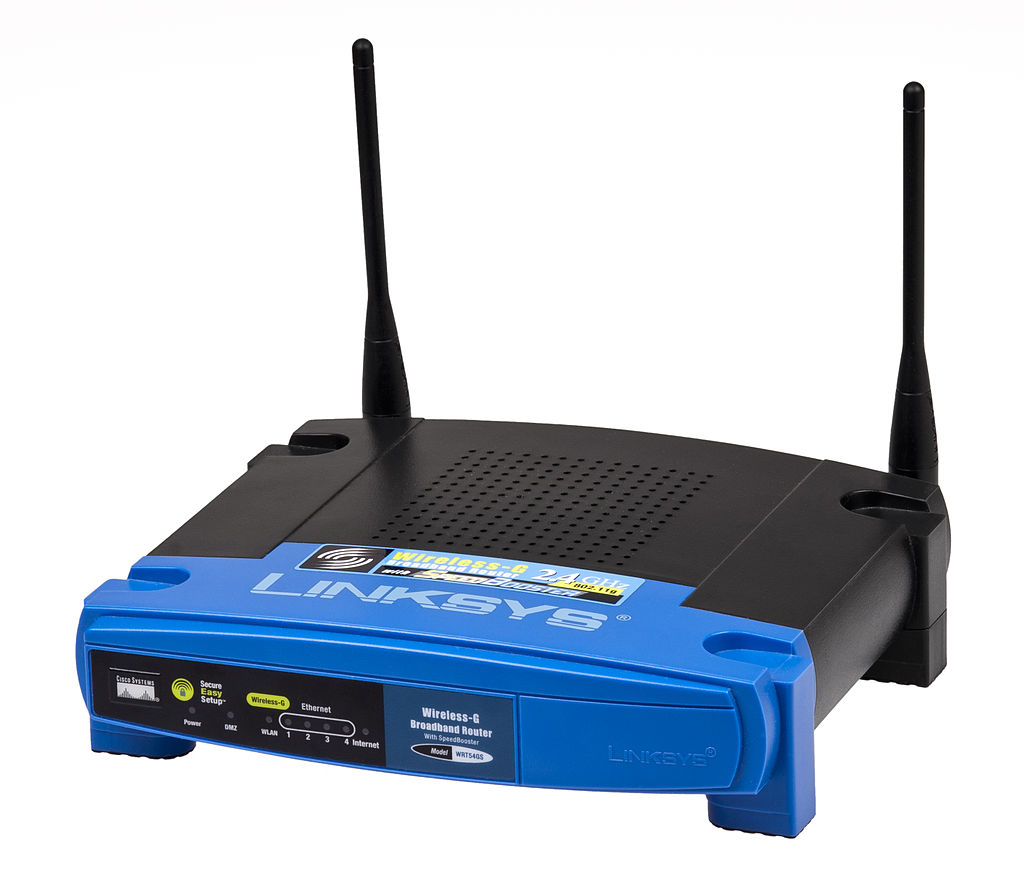
\includegraphics[height=2.8cm]{res/router.jpg}\hcite{router}
		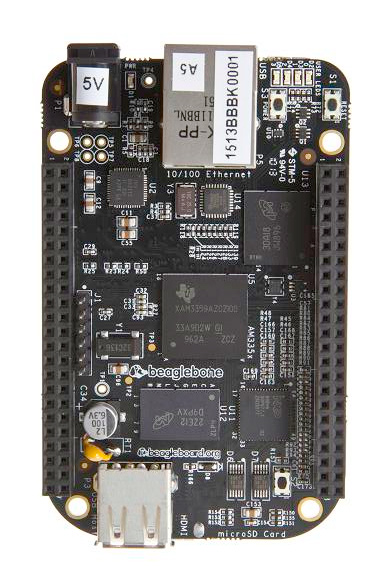
\includegraphics[height=3cm]{res/Beaglebone_Black.jpg}\hcite{beagleboneBlack}
	\end{center}
	\only<handout>{
		\begin{itemize}
			\item Industrie-Boards
			\item Consumer Hardware (Router, Media-Center, \ldots)
			\item Eval-/Bastelboards (Raspi, BeagleBone)
			\item[$\rightarrow$] BeagleBone Green
			\begin{itemize}
				\item Netzwerk
				\item Yocto Supported
				\item viele Anshlüsse
				\item USB Powered
			\end{itemize}
		\end{itemize}
	}
\end{frame}

\section{OS}

\begin{frame}{GNU/Linux Distribution}
	\begin{itemize}
		\item off-the-shelf (Debian, OpenWRT, \ldots)
		\visible<2->{
			\begin{itemize}
				\item weite Verbreitung; bekannt
				\item Updates werden von anderen bereitgestellt
				\item erlaubt Lizenz Verteilung?
			\end{itemize}
		}
		\item Yocto\hcite{whyYocto}\only<handout>{\footnote{Tools und Rezepte um eigene GNU/Linux Distribution zu bauen}}
		\visible<3->{
			\begin{itemize}
				\item git repository mit Konfiguration des gesamten System
				\item Patchen einzelner Pakete
				\item Optimierungen auf spezifische Hardware
				\item volle Kontrolle
			\end{itemize}
		}
	\end{itemize}
\end{frame}
